
\section{Theorie}
\label{sec:Theorie}

Unter dem Begriff Zeeman-Effekt wird ein Phänomen verstanden, welches Auftritt, wenn ein Atom in ein Magnetfeld gebracht wird. Aufgund der verschiedenen magnetischen Momente der Zustände des Atoms mit gleichem Energieniveau ohne anglegten Magnetfeld, kommt es im Magnetfeld zu einer Aufspaltung dieser Energieniveaus. Diese Aufspaltung wird im Spektrum in Form zusätzlicher Wellenlängen sichtbar. Von besonderer Bedeutung für diesen Effekt sind die aus den Spins und Drehimpulsen der Elektronen in verschiedenen Zuständen zusammengesetzten Gesamtdrehimpulse sowie die zugehörigen Landé-Faktoren.


\subsection{Drehimpuls, Spin und magnetisches Moment eines Elektrons}
Elektronen in der Elektronenhülle des Atoms kann sowohl ein Drehimpuls als auch Spin zugeordnet werden. Die Quantenzahlen $n$, $l$ und $s$ der Eigenzustände des Elektrons haben folgende Beziehung zu den Drehimpuls $\vec{l}$ und Spin $\vec{s}$:
\begin{align*}
	|\vec{l}|= \hbar \sqrt{l(l+1)} & \text{ mit } l=0, 1, \hdots, n-1\\
	|\vec{s}|= \hbar \sqrt{s(s+1)} & \text{ mit } s=\frac{1}{2}.
\end{align*}
Daraus ergibt sich das magnetische Moment zu:
\begin{gather*}
	\vec{\mu}_l=-\mu_\text{B} \frac{\vec{l}}{\hbar}=-\mu_\text{B} \sqrt{l(l+1)} \vec{l}_e \\
	\vec{\mu}_s=- g_\text{s} \mu_\text{B} \frac{\vec{s}}{\hbar}=- g_\text{s} \mu_\text{B} \sqrt{s(s+1)} \vec{s}_e
\end{gather*}
wobei es sich bei $\vec{l}_e$ und $\vec{s}_e$ um die jeweiligen Einheitsvektoren und bei $\mu_\text{B}=\frac{e_0 \hbar}{2 m_0}$ um das Bohrsche Magneton handelt. Die Größe $e_0$ ist die Ladung des Elektrons und $m_0$ die Masse. Die Größe $g_\text{s}$ ist der Landé-Faktor des Elektrons und is gilt $g_\text{s} \approx 2$. Dieser Unterschied beim Spin zum Bahndrehimpuls wird als magnetomechanische Anomalie des Elektrons bezeichnet und folgt aus der Dirac-Gleichung. Das gesamte magnetische Moment ist dann durch:
\begin{gather*}
	\vec{\mu}_\text{ges}= \vec{\mu}_l+\vec{\mu}_s
\end{gather*}
gegeben.

\subsection{Kopplung von Drehimpuls und Spin zum Gesamtdrehimpuls}

Wie die Drehimpulse und Spins in einem Mehrelektronensystem zum Gesamtdrehimpuls koppeln ist von System zu System verschieden und nur schwer zu behandeln. Es können jedoch zwei wichtige Grenzfälle relativ einfach behandelt werden. Der eine Grenzfall ist die LS- oder auch Russell-Saunders-Kopplung. Dies ist der Grenzfall für Atome mit kleiner Kernladungszahl. Hierbei setzen sich die Drehimpulse und Spins jeweils sich zu einem Drehimpuls \[\vec{L}=\sum_i \vec{l}_i\] und einem Spin \[\vec{S}=\sum_i \vec{s}_i\] der gesammten Elektronenhülle zusammen. Der Drehimpuls und Spin wird dabei durch die Drehimpulse und Spins in den unabgeschlossenen Schalen zusammengesetzt, da sich die Drehimpulse und Spins jeweils in den abgeschlossenen Schalen gegenseitig aufheben. Der Gesamtdrehimpuls der Elektronenhülle ergibt sich zu \[\vec{J}=\vec{L}+\vec{S}.\] Für die jeweiligen magnetischen Momente gilt:
\begin{gather*}
	\vec{\mu}_L=-  \mu_\text{B} \frac{\vec{L}}{\hbar}=- \mu_\text{B} \sqrt{L(L+1)} \vec{L}_e\\
	\vec{\mu}_S=- g_\text{s} \mu_\text{B} \frac{\vec{S}}{\hbar}=- g_\text{s} \mu_\text{B} \sqrt{S(S+1)} \vec{S}_e\\
	\vec{\mu}_J=\vec{\mu}_L+\vec{\mu}_S.
\end{gather*}

Der andere Grenzfall wird als $jj$-Kopplung bezeichnet. Dies ist der Grenzfall für Atome mit hoher Kernladungszahl. Hier koppeln die Drehimpulse und Spins der Elektronen einzeln zu den Gesamtdrehimpulsen der einzelnen Elektronen \[\vec{j}_i=\vec{l}_i+\vec{s}_i.\] Diese addieren sich zum Gesamtdrehimpuls der Elektronenhülle \[\vec{J}=\sum_i \vec{j}_i .\]



\subsection{Aufspaltung im Magnetfeld}
Es wird im Folgendem die Aufspaltung im Magnetfeld für den Grenzfall kleiner Kernladungszahlen betrachtet. Von Bedeutung für diese ist die parallel zum Magnetfeld ausgerichtete Komponente des magnetischen Momentes des Gesamtdrehimpuls der Elektronenhülle. Das gesamte magnetische Moment ergibt sich wie im vorherigem Kapitel beschrieben. Die parallel zum Gesamtdrehimpuls ausgerichtete Komponente wird mit $\vec{\mu}_J$ bezeichnet. Die senkrechte Komponente ist hier nur von geringer Bedeutung, da sie im zeitlichen Mittel verschwindet. Für den Betrag von $\vec{\mu}_J$ gilt:
\begin{align*}
	|\vec{\mu}_J|&=\mu_B \sqrt{J(J+1)} \cdot \frac{(1+g_S) J (J+1) + (g_S-1)\{S(S+1)-L(L+1)\}}{2 J (J+1)}\\
	&= \mu_B\cdot g_J \cdot\sqrt{J(J+1)},
\end{align*}
wobei der Faktor 
\begin{align*}
	g_J&=\frac{(1+g_S) J (J+1) + (g_S-1)\{S(S+1)-L(L+1)\}}{2 J (J+1)}\\
	&\approx \frac{3 J (J+1) + S(S+1)-L(L+1)}{2 J (J+1)}
\end{align*}
als Landé-Faktor bezeichnet wird. Aufgrund des Phänomens der Richtungsquantelung kann $\vec{\mu}_J$ nur Richtungen annehmen, bei welchen die Komponente $\mu_{J_{||}}$ in Entlang der Feldlinen ein ganzes Vielfaches von $\mu_B \cdot g_J$ ist. Es gilt also:
\begin{align*}
	\mu_{J_{||}}=-\mu_B g_J  \cdot m & \text{ mit } m=-J,-(J-1), \hdots, J.
\end{align*}
Es kann $|m|$ nicht größer als $J$ werden, da der Betrag vom Gesamtdrehimpuls immer größer als der Betrag einer Komponente ist. Damit gibt es $2 J +1 $ verschiedene mögliche Einstellungen des Gesamtdrehimpuls bezüglich des Magnetfeldes. Jede Einstellung im Magnetfeld entspricht einer potentiellen Energie. Es gilt:
\begin{gather*}
	E_{m}=-\vec{\mu_{J}} \cdot \vec{B} = -\mu_{J_{||}} \cdot B= \mu_B g_J B \cdot m.
\end{gather*}
Damit gibt sich für die Energie der Energieniveaus nach Aufspaltung im Magnetfeld eines Energieniveaus:
\begin{gather}
	E=E_{m}+E_0=\mu_B g_J B \cdot m +E_v, \label{eq:ENiveau}
\end{gather}
wobei $E_v$ die Energie des Energieniveaus vor der Aufspaltung bezeichnet.
Es ergibt sich z.B. die in Abbildung \ref{fig:generelleAufspaltung} dargestellte Aufspaltung eines Energieniveaus.
\begin{figure}
	\centering
	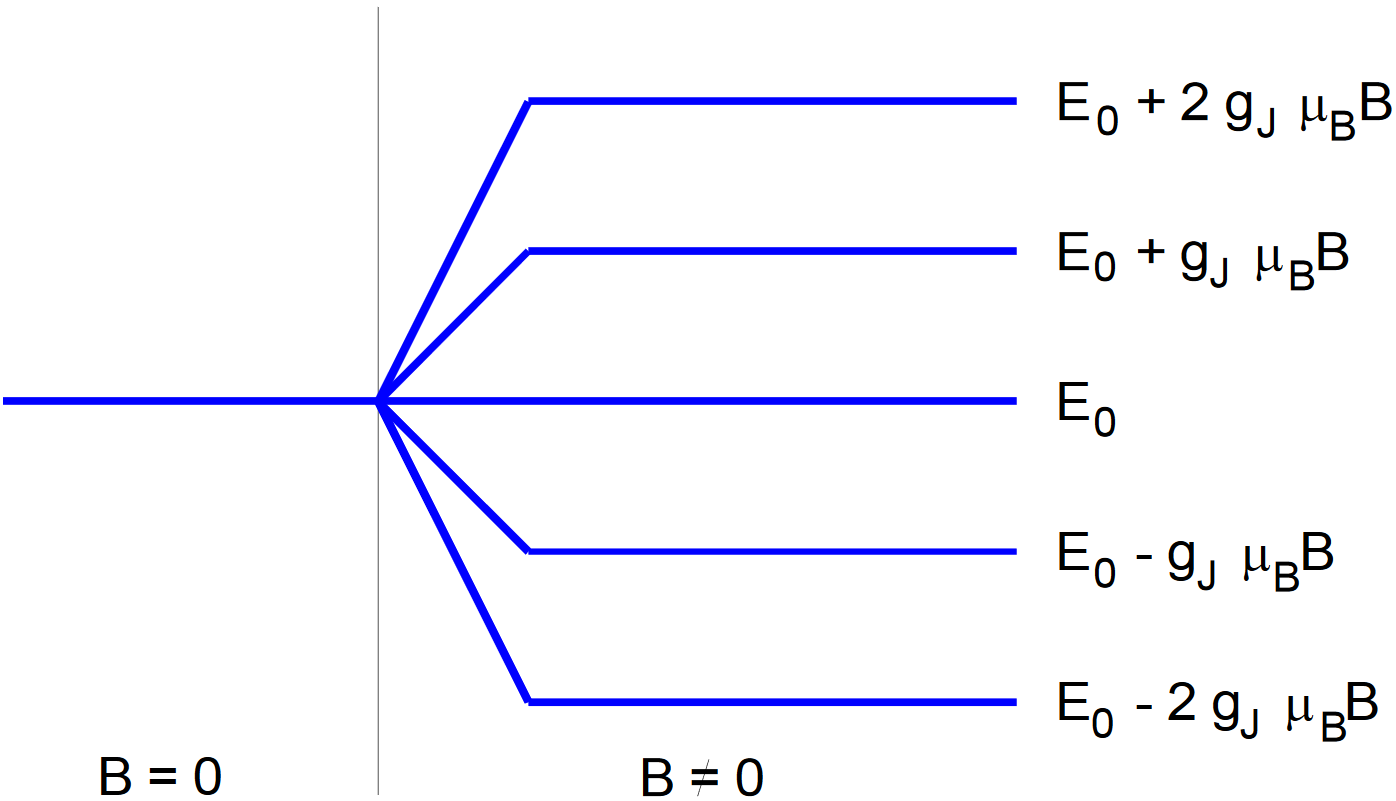
\includegraphics[width=\linewidth-150pt,height=\textheight-150pt,keepaspectratio]{content/Images/generelleAufspaltung.png}
    \caption{Theoretische Aufspaltung eines Enegieniveaus eines Atoms mit $J=2$ im Magnetfeld \cite{V27}.}
    \label{fig:generelleAufspaltung}
\end{figure}

\subsection{Auswahlregeln für Übergänge zwischen Zuständen}
Zwischen den aufgespaltenen Energieniveaus kann es zu Übergängen kommen. Es sind jedoch nicht alle Übergänge gleich wahrscheinlich. So gibt es verbotene Übergänge, die stark unterdrückt sind. Aus der Lösung der zeitabhängigen Schrödinger-Gleichung ergibt sich folgende Regel: 
\begin{gather*}
	\Delta m =0, \pm 1,
\end{gather*}
wobei sich für $\Delta m=0$ linear zum Magnetfeld und für $\Delta m=\pm 1$ zirkular um die Magnetfeldrichtung polarisierte Strahlung ausbildet. Die linear polarisierte Strahlung wird als $\sigma$-Komponente und die linear zur Feldrichtung polarisierte Strahlung als $\pi$-Komponente bezeichnet. Die $\sigma$-Komponente besitzt demnach eine longitudinale und eine transversale Komponente, wobei die transversale Komponente senkrecht auf der transversalen Komponente der $\pi$-Komponente steht. Es ergibt sich folgend die in Abbildung \ref{fig:linien} dargestellten Linien bei longitudinaler und transversaler Beobachtung.
\begin{figure}
	\centering
	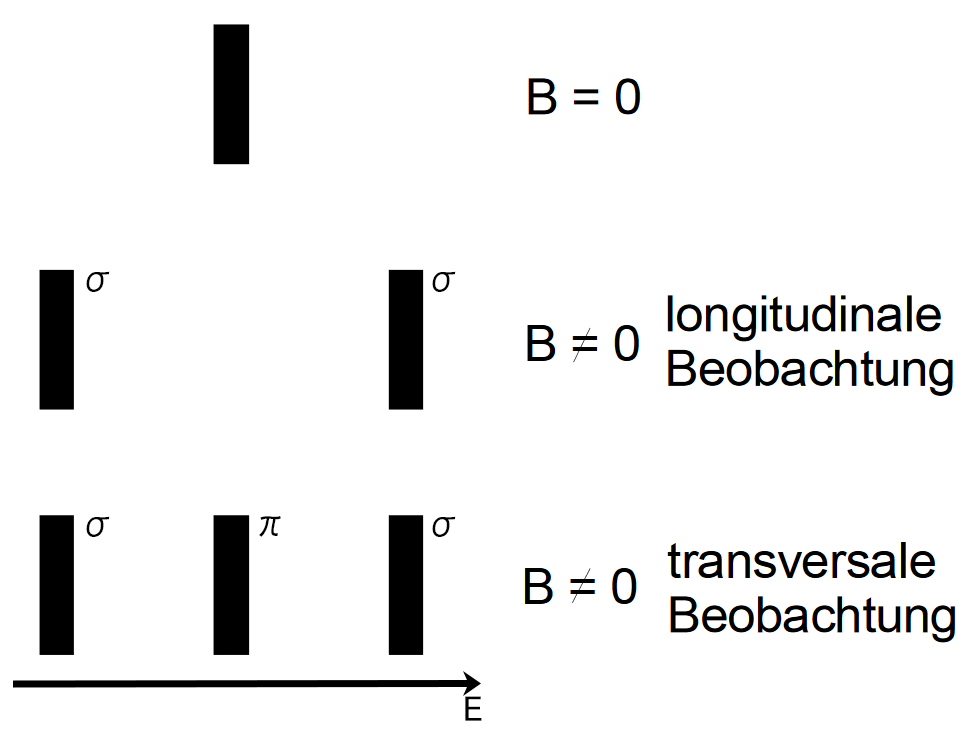
\includegraphics[width=\linewidth-150pt,height=\textheight-150pt,keepaspectratio]{content/Images/linien.png}
    \caption{Theoretische Spektrallinien ohne und mit Magnetfeld für den in Abbildung \ref{fig:normaleAufspaltung} dargestellten Fall in longitudinaler und transversaler Beobachtung \cite{V27}.}
    \label{fig:linien}
\end{figure}


\subsection{Der Zeeman-Effekt}
Die zuvor diskutierten Übergänge können nun zwischen Zuständen mit Spin (anomaler Zeeman-Effekt) und zwischen Zuständen ohne Spin (normaler Zeeman-Effekt) auftreten. Für die Energie des, beim Übergang vom höheren ins niedrigere Energieniveau, emitierten Photons ergbibt sich allgemein:
\begin{align*}
	E_\gamma &= \Delta E = E_2-E_1 \\
	&=\{g_{J_2} \cdot m_2-g_{J_1} \cdot m_1 \} \mu_B B  + E_0,
\end{align*}
wobei $E_0$ die Energie des emitierten Photons ohne Aufspaltung im Magnetfeld bezeichnet.
Für den Fall des normalen Zeeman-Effektes gilt $g_{J}=1$ und es lässt sich deshalb die Formel vereinfachen zu:
\begin{align*}
	E_\gamma = \mu_B B \cdot \Delta m +E_0.
\end{align*}
Folglich gibt es beim normalen Zeeman-Effekt aufgrund der Auswahlregel nur zwei neue Spektrallinien (für $\Delta m = -1$ und $\Delta m = +1$). Dies ist beim anomalen Zeeman-Effekt im Allgemeinen nicht der Fall (z.B. in Abbildung \ref{fig:anomaleAufspaltung}). Ein möglicher Fall für den normalen Zeeman-Effekt ist in Abbildung \ref{fig:normaleAufspaltung} dargestellt.
\begin{figure}
	\centering
	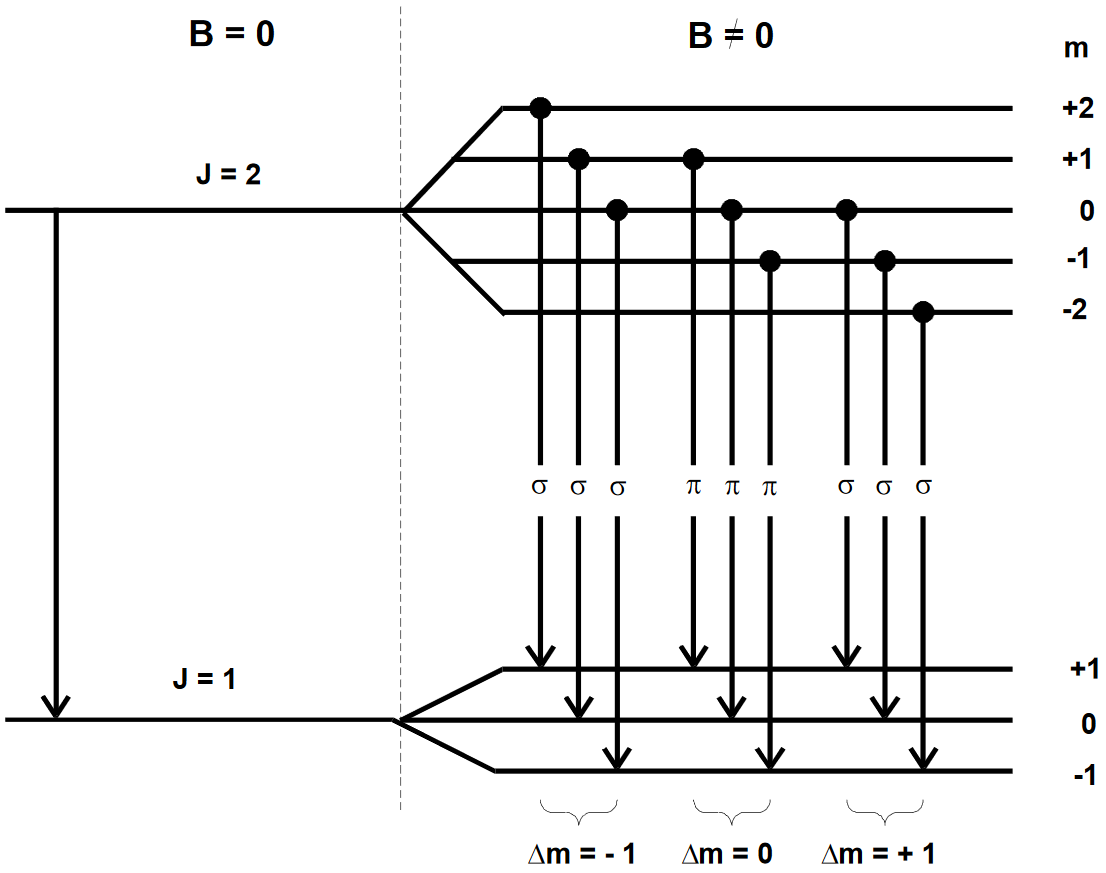
\includegraphics[width=\linewidth-150pt,height=\textheight-150pt,keepaspectratio]{content/Images/normaleAufspaltung.png}
    \caption{Aufspaltung und Polarisation der Spektrallinien beim normalen Zeeman-Effekt ($S = 0$) \cite{V27}.}
    \label{fig:normaleAufspaltung}
\end{figure}
\begin{figure}
	\centering
	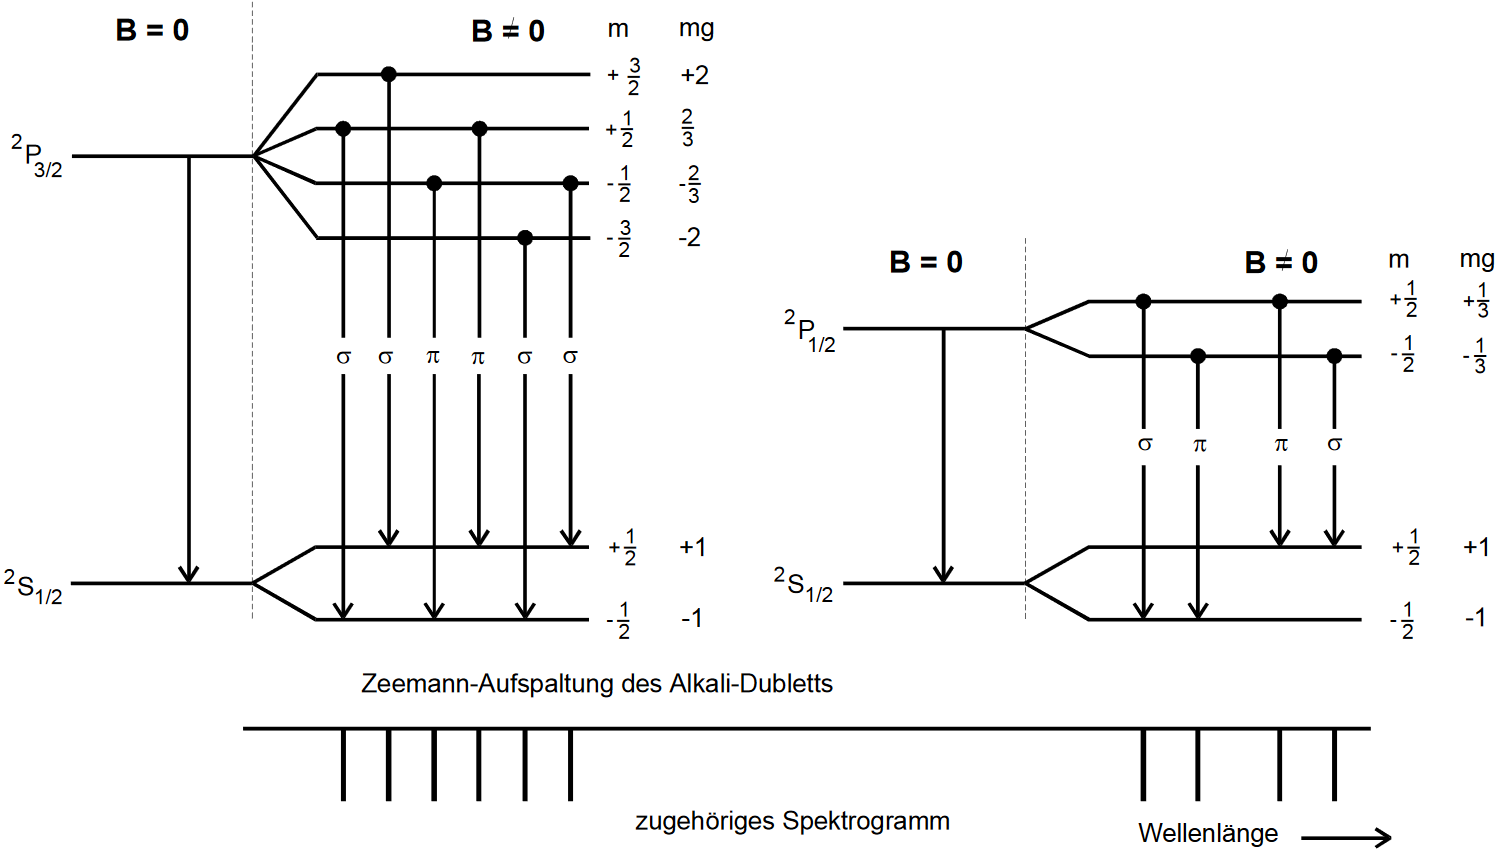
\includegraphics[width=\linewidth-50pt,height=\textheight-50pt,keepaspectratio]{content/Images/anomaleAufspaltung.png}
    \caption{Beispiel einer Linienaufspaltung beim anomalen Zeeman-Effekt. Dargestellt ist die Aufspaltung eines Alkali-Dubletts \cite{V27}.}
    \label{fig:anomaleAufspaltung}
\end{figure}